\renewcommand{\thesection}{\Alph{section}}
\section{Product perspective}\label{sec:product_perspective}
\subsection{Scenarios}\label{subsec:scenarios}
\subsubsection{Scenario 1: Mr.Spongebob registers on the platform}\label{subsubsec:scenario_1}
Mr.Spongebob, a final-year student at the University of Bikini Bottom, is looking for an internship to practice the knowledge he's gained. 
To do so, he asks advice from Professor Puff, who suggests using the Students\&Companies platform to search for internship opportunities.
Following her advice, Mr.Spongebob registers as a student on the platform, selecting the University of Bikini Bottom from the list of 
universities and verifying his student status with his educational email and password. Then, he fills in all the required personal information,
including his name, date of birth, and other details. He also inserts keywords to describe his skills and the job fields he might be interested 
in. Finally, after uploading his CV, which contains all the necessary information and details, Mr.Spongebob completes his registration and 
can begin searching for internships. Meanwhile, Professor Puff, who oversees internship activities using the official account of the University of 
Bikini Bottom, is notified of Mr.Spongebob's registration.

\subsubsection{Scenario 2: Mr.Krabs publishes an internship offer}\label{subsubsec:scenario_2}
Due to the rapid evolution of Technology, Mr.Krabs decides to collaborate with his competitor Mr.Plankton, on a new project. They
plan to develop a ``Hamburger super secret formula detector'' that can detect what the customer likes by looking at his facial expressions, in 
order to to create the perfect personalized hamburger! To achieve this, they need to hire students specializing in Computer Vision, Deep Learning and
AI to study the visual data. So Mr.Krabs logs into the Students\&Companies platform using the official company account
and navigates to the ``Publish Internship'' section to create a new announcement. He fills in all the required information: 
the title, location, role, application deadline, number of positions, duration, employment type, description, and required skills. \\
\begin{quote}
    \begin{center}
       \textbf{\textquotedbl{}Computer Vision and AI Intern\textquotedbl{}}
    \end{center}
    
    \textit{Location:} Krusty Krab Technology Lab, Bikini Bottom \\
    \textit{Role:} Intern \\
    \textit{Application Deadline:} 25th December 2024 \\
    \textit{Number of Positions:} 2 \\
    \textit{Duration:} 6 months \\
    \textit{Employment Type:} Full-time \\
    \textit{Description:} We are looking for students who can contribute to the development of the Hamburger super secret formula detector by developing 
    algorithms that collect and analyze visual data. A love for hamburgers is essential!\\
    \textit{Required Skills:} Computer Vision, AI, Python, Deep Learning
\end{quote}
After that, Mr.Krabs publishes the internship offer, which can be seen in the ``Available Internships'' section and in the company's profile section. 
Immediately after the publication, he receives a notification of recommended student profiles that may match the offer requirements.


\subsubsection{Scenario 3: Mr.Patrick searches for internships}\label{subsubsec:scenario_3}
Mr.Patrick is very worried because he is in the last semester of his master's degree, so he has to find an internship or he won't be able to graduate in Food Engineering.
He remembers he has an account on the Students\&Companies platform, which he used to find an internship at the beginning of his studies, so he decides 
to take another look at the platform. He logs in and updates his profile and CV, adding the new skills he has acquired during his master’s degree.
He navigates to the search bar and types ``Hamburger'' to look for internships related to hamburger studies. When he doesn’t find anything that 
interests him, he scrolls through the recommended internships list. Finally, he finds Mr.Krabs' posting and becomes very interested in the 
project, so he applies for the internship and waits for the company's response. After applying, he can check the status of his application in 
the ``Your Applications'' section.

\subsubsection{Scenario 4: Krusty Krab Technology Lab Interview}\label{subsubsec:scenario_4}
After the application deadline, Mr.Krabs and Mr.Plankton review all the applications received for the intern position. They select the
candidates by reviewing their profiles and CVs, and then send them an invitation for an interview. For the first round of interviews, Mr.Plankton
decides to formulate a set of short questions to know more about the candidates' skills and experiences. The candidate will be able to respond to 
these questions through a form inside the platform. In said form Mr.Plankton also includes the date, time and location of the interview and the 
necessary information to better prepare the candidates. After sending the invitations, the candidates selected for the interview receive a notification 
from the platform. At the end of the interview, Mr.Plankton evaluates the candidates and discusses with Mr.Krabs to decide who to hire. Finally, they 
send an offer to the best candidates and wait for their acceptance to start the internship.

\subsubsection{Scenario 5: Mr.Gary's application is rejected}\label{subsubsec:scenario_5}
Mr.Gary, an undergraduate student at the University of Bikini Bottom, applied for an internship at the ``Krusty Krab Technology Lab'' since he was very 
interested in the internship opportunity. After the application deadline, Mr.Krabs and Mr.Plankton reviewed all the applications received for the intern 
position. Unfortunately, they do not think Mr.Gary has enough experience for the internship, so they reject his application. Mr.Gary received a 
notification informing him that his application was not selected and explaining the reason for the decision. He will still be able to see his application 
in the ``Your Applications'' section and the status will be marked as ``rejected''.

\subsubsection{Scenario 6: Mr.Squidward goes through the interview phase}\label{subsubsec:scenario_6}
Mr.Squidward, a student at the University of Bikini Bottom, was selected for an interview after he applied to the ``Krusty Krab Technology 
Lab'' as a data science intern. He goes to the ``Your Applications'' section and fills the interview form with his answers. Then he checks the details for the 
live interview and prepares for it. In the meantime, he can communicate with the company through the chat system to ask questions, clarify any doubts or 
reschedule the interview if needed. After the interview, he receives feedback from the company about his performance and waits for the final decision. 
Finally, if he is selected he will receive a notification with the offer from the company, he can still choose to turn down the offer if he changes 
his mind or finds a better opportunity, in that case, the chat will be deactivated. Otherwise, if he accepts the internship will start and the chat 
will remain active.

\subsubsection{Scenario 7: Ms.Sandy starts her internship}\label{subsubsec:scenario_7}
Ms.Sandy is very passionate about space and is thrilled to have been selected for an internship at the Underwater Space Agency. She receives 
and accepts an offer from the company. At the same time, the Bikini Bottom University of Aerospace's professor Manta received the notification
about the new activity started by Sandy. However, she is a bit anxious, so she logs into the platform and navigates to the ``Internship'' 
section to review its details and opens the chat with the company's representative. She then asks some questions about how she should prepare in the 
coming days and for any advice that they think should be useful to know to have a good start in the internship.

\subsubsection{Scenario 8: Mr.Squidward leaves his feedback}\label{subsubsec:scenario_8}
At the end of his internship at the ``Krusty Krab Technology Lab'' as a data science intern, Mr.Squidward is surprised by the experience 
he has gained, even though he has several complaints about the heavy workload. He decides to leave a warm message for Mr.Krabs and Mr.Plankton 
to thank them for the opportunity. After that, he navigates to the ``Internship'' section to add a review of his internship experience and rate 
the company. It is also the section where he can check the suggestions left by his mentors regarding his internship, which is only visible to the 
company and the university.

\subsubsection{Scenario 9: Track the internship activities}\label{subsubsec:scenario_9}
As the internship period progresses, Professor Puff is responsible for overseeing the students' activities at the University of Bikini Bottom. 
She is curious to know how the students are doing in their internships, particularly Mr.SpongeBob, who is using the platform for the first time. 
She logs into the platform with the university credentials and looks at the list of students, searching for SpongeBob's name. She finds, 
in his active internship section, that he has been selected for an internship at the ``Krusty Krab Technology Lab''. By reading the feedback 
left by the company throughout the different stages of the internship, she is very glad to see that SpongeBob is doing well in the field he is 
passionate about!


\subsection{Domain-level diagram}\label{subsec:domain_level_diagram}
\begin{figure}[H]
    \centering
    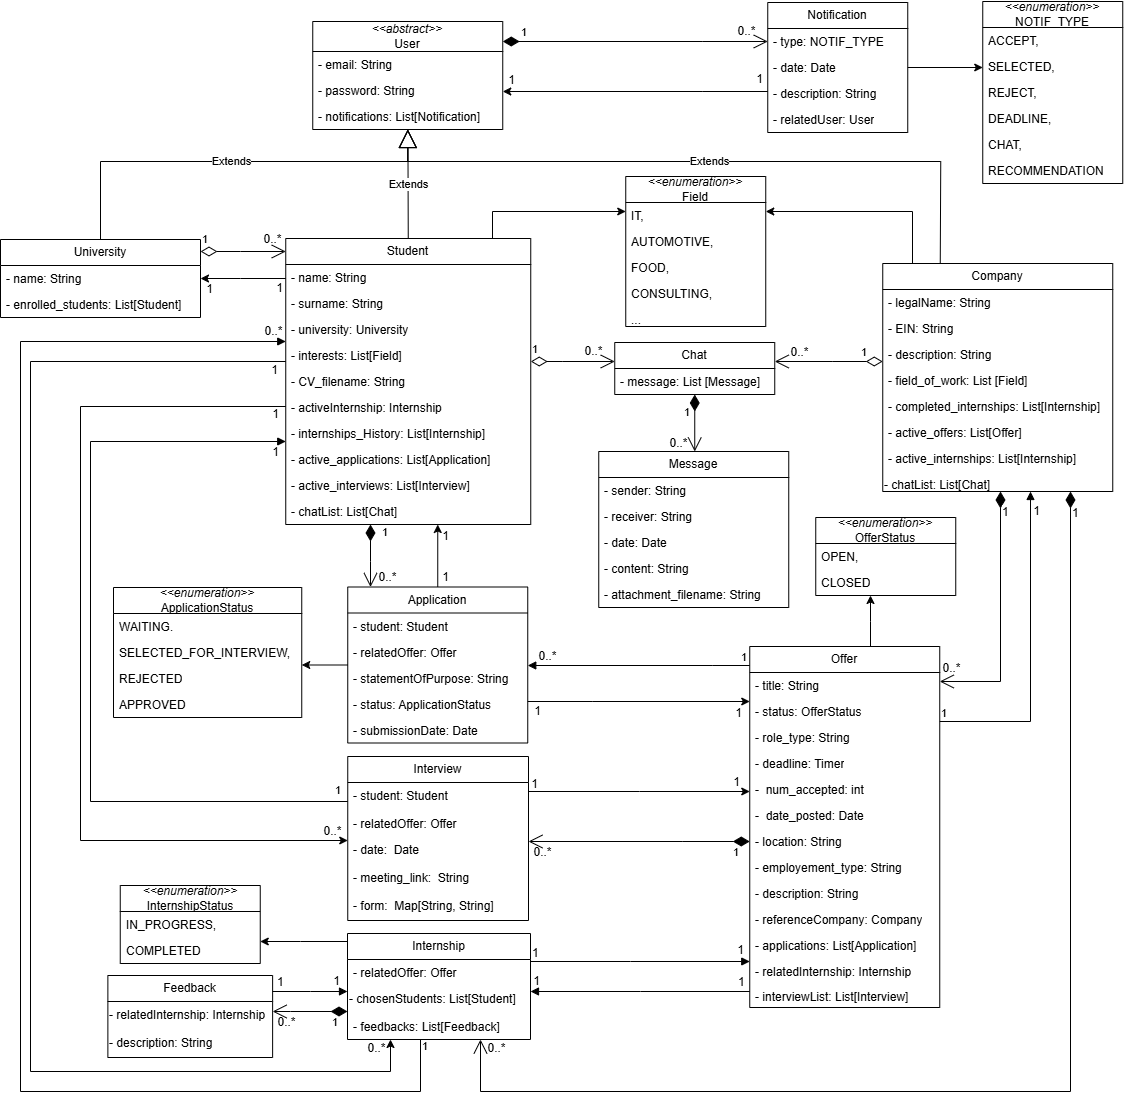
\includegraphics[width=1\textwidth]{Images/UML_Class_diagram.png}
    \caption{Domain-level diagram}\label{fig:domain-lebel_diagram}
\end{figure}
Students, Companies and Universities are implemented by extending the abstract class User. The User class contains the common attributes: email, password and
the list of notifications. Notifications have a type, description and date and are related to a specific User. Universities have a name and contain the list 
of all their enrolled students. The Student class contains specific attributes to save their profile information (like name, interests, university, CV) and 
can create applications for internships that are stored in a list. They also have references to current interviews for internships, current chats and ongoing 
and past internships. Companies contain specific attributes to save their profile information (like legalName, EIN, field of work) and can create internships 
that are stored in a list. They also have references to ongoing and past internships, currently active offers and current chats. \\
The chat is a collection of messages between a sender and a receiver. \\
The Application class contains the information about the student that applied for an internship's offer, their personal statement of purpose and also records 
the status of the application. The Offer class contains all the information about the internship: the title, location, description, deadline. It also has
references to the Company who made the proposal, the Internship itself and maintains a list of all the submitted applications and all the interview sessions.\\
The Interview class contains the information about the interview session: the date and link to the live session, and the map containing both the questions and 
the student's answers. The Internship class contains a reference to the related Offer, a list of the students that were chosen for the internship, and a list of
the feedbacks left both by the students and the company at the end of it. The Feedback class contains a reference to the related Internship and a description.\\
There are enumerations to keep track of the state of the Application, Internship and Offer.

\subsection{Statecharts}\label{subsec:statecharts}
The following sections present statechart diagrams for the platform's main processes, including internship recommendations, the internship 
selection process, and internship status tracking. 

\subsubsection{1. Internship recommendation}\label{subsubsec:internship_application}
\begin{figure}[H]
    \centering
    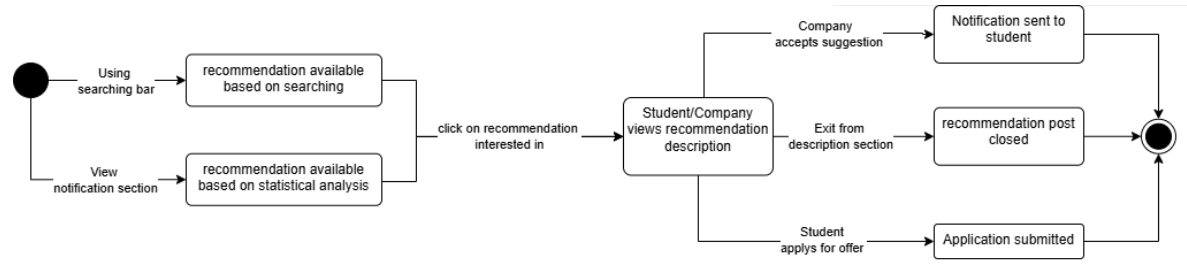
\includegraphics[width=1\textwidth]{Images/Internship_recommendation.png}
    \caption{Statechart diagram for internship recommendation}\label{fig:statechart_internship_recommendation}
\end{figure}
The recommendation process is a key functionality of the platform. After logging in, both students and companies can use the search system to view 
recommendations that match their preferences. Alternatively, they can access suggestions in the notification section, which are generated through
a statistical analysis of data from profiles and internship details. As illustrated in the statechart diagram, when users find an interesting 
recommendation, they can click on it to view more details. At this stage, students can apply for the internship, while companies can decide whether
to accept the student profile. If accepted, the student will be notified that a company is interested in their profile for a specific internship. 
Otherwise the student or the company can close the recommendation after reviewing it.

\subsubsection{2. Selection process for internship}\label{subsubsec:internship_feedback}
\begin{figure}[H]
    \centering
    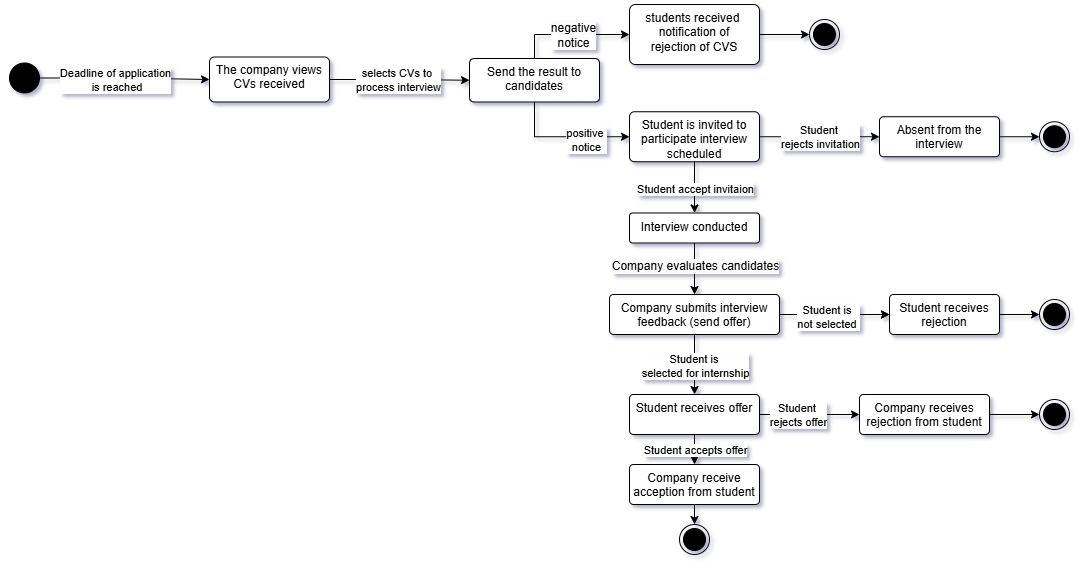
\includegraphics[width=1\textwidth]{Images/Selection_process.png}
    \caption{Statechart diagram for selection process for internship}\label{fig:statechart_selection_process_for_internship}
\end{figure}
With the selection process, after the application deadline, companies will review all applications received for the intern position and select 
candidates for the interview stage. Once a decision is made, the company will send an interview invitation to the selected candidates through 
the platform, while those not selected will receive a notification explaining that, unfortunately, they were not chosen to proceed further.
For selected candidates, a chat system between the company and the candidate will be activated to allow both parties to communicate and schedule 
interview details. If a candidate does not attend the interview, the company will consider this as a rejection of the invitation.
After all interviews are completed, the company will evaluate the candidates and decide whom to hire. The selected candidates will receive an offer, 
and the company will await their acceptance to confirm the internship role. At the same time, candidates not selected at this stage will receive a 
rejection notification. Once candidates respond to the offer, the company will be notified of their decision.

\subsubsection{3. Internship status}\label{subsubsec:monitoring_student_activities}
\begin{figure}[H]
    \centering
    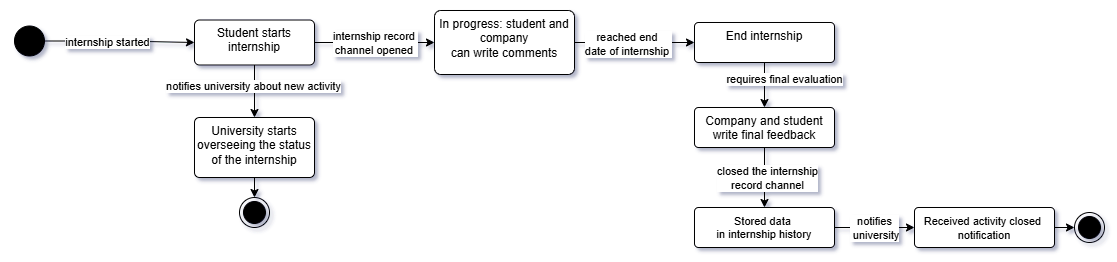
\includegraphics[width=1\textwidth]{Images/Internship_status.png}
    \caption{Statechart diagram for internship status}\label{fig:statechart_internship_status}
\end{figure}
This statechart diagram will illustrate the internship status tracking process. Once the internship begins, the student’s university will be notified, 
allowing the university to monitor the student’s activities and ensure the internship is progressing as expected.
During the internship, the student can use a chat feature to communicate with their mentor and provide feedback on their internship experience in the 
specific internship section. Similarly, the company can use the chat to communicate and leave feedback on the student’s performance, offering suggestions
for improvement.
At the end of the internship, both the student and the company must complete the final evaluation and feedback process, marking the end of the internship phase.
The internship will then be officially closed, and all related information will be archived in the database. At this stage, the university will be notified
of the internship’s completion.
The student will find this internship listed as a past activity in their internship history, and the company will have access to this record in their records
 for future reference.

\section{Product functions}\label{subsec:product_functions}
\begin{itemize}[label={ }]
    \item \textcolor{bluepoli}{\textbf{Sign up and login}} 
    \\There are three types of users on the platform: students, companies, and universities. The platform allows users to create an account if they do not already 
    have one. In the first step, each user will be prompted to specify whether they are a student, company, or university. All users will need to set up login
    credentials with an email address and password.
    For students, the system will ask them to select their university from a list. If their university is not listed, they will be unable to continue with
    registration. Students must also verify their status by using their educational email.
    For companies, multiple accounts can be created under the same organization, with each linked to a different department’s unique email address. The 
    company’s identity shall be also verified using its unique EIN number and other required details.
    Once verified, users can access the platform with their email and password. On first login, the system will require users to complete their profile with
    essential information to finalize registration. Students, in particular, must upload a CV before accessing other features of the platform.
    After registration, users can log in simply by selecting their user type and entering their credentials.

    \item \textcolor{bluepoli}{\textbf{Data management system}}
    \\ The platform securely stores all user data in a protected database, including personal information, CVs, chat history, and other relevant data. 
    Specifically, the system retains detailed internship information, such as announcements, applications, interview records, internship status, and 
    feedback, which are used to analyze and optimize the matching algorithm. Additionally, other user data is recorded to provide better personalized 
    recommendations and notifications. The system ensures that all data is encrypted and protected from unauthorized access.
    Furthermore, users have the option to delete their accounts, modify personal information, and, for students, update their CVs as needed.

    \item \textcolor{bluepoli}{\textbf{Search system}}
    \\This function allows students to search for internships using keywords such as job title, company name, location, and more. Similarly, companies 
    can search for student profiles using criteria like name, university, skills, and other relevant details. Universities, on the other hand, can 
    search a specific student within their student list by name to monitor activities and access the student's profile.
    The search system will display a list of recommendations based on the user's preferences and search history. Additionally, users can filter the
    search results by selecting specific categories to refine their search.

    \item \textcolor{bluepoli}{\textbf{Recommendation system}} 
    \\This feature is one of the platform's main functionalities, offering personalized recommendations to students and companies based on their search
    preferences and the statistical analysis of data from profiles and internship details. Recommendations can be viewed in the search results or in 
    the notification section.
    The system is designed to continuously improve the accuracy of these recommendations by analyzing user behavior and feedback in real-time, 
    optimizing the quality of the results. Users can click on a recommendation to view more details about the internship posting or student profile.

    \item \textcolor{bluepoli}{\textbf{Internship application}}
    \\Through this function, students can apply for internships that interest them after viewing the details of the posting. Once the application deadline
    has passed, the company will review all received applications and select candidates for the interview stage. The platform will notify students of 
    the results at this phase. 
    If a student's application is accepted, they will be invited for an interview. Otherwise, the student will be notified that their application was rejected.
    However, the student can still apply for other internships, but cannot reapply for the same internship once rejected.
    \item \textcolor{bluepoli}{\textbf{Internship Posting}}
    \\Companies can publish internship offers on the platform using this function. In the ``Publish Internship'' section, companies must provide all required
    details, including the title, location, role, application deadline, number of positions, duration, employment type, description, and required skills.
    Once the internship offer is published, the company will receive recommendations for student profiles that match the offer’s criteria. Additionally, 
    the company can access the ``Available Internships'' section and select a specific posting to view the list of applications received and select 
    candidates for the interview stage.

    \item \textcolor{bluepoli}{\textbf{Selection phase Assistance}}
    \\Once the application deadline has passed, the company can use this function to select candidates and send interview notifications. The system will 
    guide the company through the selection process by providing a list of received applications, allowing the company to review each candidate's profile 
    and CVs. Additionally, the system will offer a chat feature and tools such as questionnaire forms to help the company know more about the candidates
    before the actual interview will take place.
    The system will also notify students of the results from the selection phase (application or interview result). If selected for an interview, the chat
    system will be activated for the student, enabling both parties to communicate and schedule interview details.

    \item \textcolor{bluepoli}{\textbf{Internship Status Tracking}}
    \\This function allows users to monitor the progress of internships, including the past completed internships and the current active internships.
    Students can view internship status through their internship history, while companies can access it through their records of the history of their 
    published internships. Universities can monitor student activities through the student list associated with them. The status tracking system
    is designed to record all important information about the internship and notify the relevant parties of any changes or updates.

    \item \textcolor{bluepoli}{\textbf{Internship Feedback system}}
    \\This feature is activated when the internship begins. Each specific internship will have a dedicated area for both the student and the company to
    provide feedback and evaluations.
    It allows students and companies to share useful information, such as suggestions, key issues, and ongoing feedback, separate from the chat system. 
    This section is designed to record important highlights throughout the internship process. At the end of the internship, the system will prompt both 
    the student and the company to submit their final evaluations or comments. Once the internship is concluded, this feature will be deactivated, and 
    all related information will be archived in the database. The university will evaluate the student's status based on the information provided by this
    feature.
    \item \textcolor{bluepoli}{\textbf{Chat system}}
    \\The chat system is an important feature of the platform that allows users to communicate with each other. Unlike a typical chat system, this function
    is not always active. It is activated once a company selects a student as a candidate for an interview to discuss interview details. 
    If the student is not selected for the final offer or rejects the offer, the specific chat window will be deactivated after the interview. However, 
    if the student accepts the internship offer, the chat system will remain active, allowing both parties to communicate during the internship period and 
    maintain contact afterward for potential future collaboration, such as mentorship or networking.
    Through the chat system, they can exchange messages and files, while the chat history will be stored in the database for future reference and analysis.
    The activation and deactivation of the chat system ensures privacy and security, preventing unnecessary communication, such as spam or harassment, 
    before real collaboration begins and filtering out unqualified messages.
    The key difference between the chat system and the feedback system is that the chat system is real-time and private, accessible only to the two parties 
    involved. In contrast, the information collected through the feedback system is more formal and public. The university can access this data when evaluating
    the student's performance, and other users can read anonymous comments left by students who participated in internships when reviewing a company's reputation.

    \item \textcolor{bluepoli}{\textbf{Notification system}}
    \\This function creates a channel for the platform to send notifications to users. Notification types include recommendations, application results,
    interview invitations, interview results, internship status updates, and other important communications from the platform. For example, when a student
    start an internship, the university will be notified through the notification system.

    \item \textcolor{bluepoli}{\textbf{Acceptance and Rejection}}
    \\This function allows users to express their decisions: students can accept or reject internship offers, and companies can accept or reject student applications.
    Once a student accepts an offer, the company is notified, and the internship officially begins. If a student rejects an offer, the company is notified, and the 
    reserved position is reopened for other candidates. Similarly, if a company rejects a student’s application, the student is notified, and the application is 
    marked as rejected.
    The acceptance and rejection system ensures that both parties are informed of the results and can proceed accordingly. Additionally, this system helps 
    improve the platform's matching algorithm by providing better recommendations in the future, based on the acceptance and rejection rates to better understand 
    user preferences.
\end{itemize}

\section{User characteristics}\label{subsec:user_characteristics}
This section will examine the needs of the platform's primary users: students, companies, and universities. 
Each user group has specific requirements, and the platform is designed to meet these needs with various features. 
Here’s an overview of what each group expects from the platform:

\subsection{Students}
Students are the primary users of the platform who are looking for suitable internship opportunities to gain practical experience. They need an intuitive and 
user-friendly interface that makes it easy to search for internships. Since many students are not familiar with the job market, they require a recommendation 
system that suggests internships match their skills, preferences, and career goals. They also expect through the platform they will be able to apply for internships
that are interested in and to update their profile and CV when they gain new skills or experiences.
Furthermore, students want to communicate directly with companies once a collaboration is established. They would like to receive feedback from companies about 
their performance during the internship, as this helps them improve their skills and future careers. Additionally, they want to share their experiences and 
leave comments to help other students evaluate potential employers before applying.
Finally, students need to be able to track the status of their internships and receive timely notifications, allowing them to take informed action.

\subsection{Companies}
Companies are the users of the platform that provide internship opportunities to students. They require a platform that allows them to easily publish and 
manage internship postings, receive applications, and select candidates for interviews. Specifically, companies expect the platform to offer recommendations 
that match the requirements for the internships they’ve posted. This helps them identify the most suitable candidates and streamline the selection process.
Companies also need an efficient communication system to interact with students for scheduling interviews and discussing internship details. 
They expect to receive feedback from students on how to improve the company’s internship programs and provide evaluations on student performance.
Additionally, companies need access to student profiles and CVs to identify the best candidates for the internships. 
They require the ability to track the status of internships and receive notifications regarding students' decisions on whether to accept or decline an offer.
The platform should allow companies to have multiple accounts, especially if they represent different departments, and manage them separately. 
Furthermore, companies should be able to select student profiles that interest them and contact students through the notification system to promote their 
internship offers.

\subsection{Universities}
As users who are closely related to the students, universities need to be able to monitor the activities of students who are registered as their students.
They need to be able to track students' internship statuses and receive notifications about updates to students' activities. Additionally, they need to 
be able to view students' profiles and activity histories to evaluate their performance, using the search bar to find a specific student.

\section{Assumptions,dependencies and constraints}\label{subsec:assumptions_dependencies_constraints}
\subsection{Domain Assumptions}
[A1] The university of the student who want to register on the platform must be listed in the platform's database. If the university is not listed, the student
will not be able to complete the registration process.

[A2] The company that wants to register on the platform have a unique EIN number available.

[A3] All students have an educational email that can be used to verify their student status.

[A4] All students should have a CV that contains all the necessary information and details about their experience.

[A5] All university have an official email that can be used to verify their identity.

[A6] Every department of a company has a unique email address that can be used to verify their identity.

[A7] The platform will be able to communicate correctly with email servers to send notifications to users.
